% !TEX TS-program = pdflatex
% !TEX encoding = UTF-8 Unicode
% ORIGIN URL
% {{{ setup

\documentclass[11pt,twoside]{article}

\usepackage[utf8]{inputenc}

\usepackage[pdftex,
            pdfauthor={AUTHOR},
            pdftitle={TITLE},
            pdfsubject={SUBJECT},
            pdfkeywords={},
            pdfproducer={},
            pdfcreator={pdflatex},
            breaklinks]{hyperref}

\usepackage{sectsty}
\allsectionsfont{\sffamily\mdseries\upshape}

\usepackage[a4paper,margin=2.5cm,headheight=13.6pt]{geometry}
\usepackage{fancyhdr}
\pagestyle{fancy} % options: empty, plain, fancy
\renewcommand{\headrulewidth}{0pt}
\lhead{}\chead{}\rhead{}
\lfoot{}\cfoot{\thepage}\rfoot{}

\usepackage{url}
\usepackage{breakurl}

\usepackage{cite}

\usepackage{placeins}
\usepackage{subcaption}
\usepackage{multirow}
\usepackage{appendix}

\usepackage{color}
\definecolor{dkgreen}{rgb}{0,0.6,0}
\definecolor{gray}{rgb}{0.5,0.5,0.5}
\definecolor{mauve}{rgb}{0.58,0,0.82}
\hypersetup{
    colorlinks,
    citecolor=black,
    filecolor=black,
    linkcolor=black,
    urlcolor=black
}

\usepackage{listings}
\lstdefinelanguage{none}{
  identifierstyle=
}
\newcommand{\lstNone}{
    \lstset{language=none,
            numbers=left,
            showstringspaces=false,
            numberstyle=\tiny\color{gray},
            numbersep=5pt,
            breaklines=false,
            basicstyle=\scriptsize\ttfamily}
}

\newcommand{\lstC}{
    \lstset{language=C,
            numbers=left,
            showstringspaces=false,
            numberstyle=\tiny\color{gray},
            keywordstyle=\color{blue},
            commentstyle=\color{dkgreen},
            stringstyle=\color{mauve},
            numbersep=5pt,
            breaklines=false,
            basicstyle=\small\ttfamily}
}

\usepackage{graphicx}
\usepackage{tikz}
\usetikzlibrary{shapes, shapes.arrows}

\usepackage{amsmath}
\usepackage{amssymb}
\newcommand{\indep}{\perp\!\!\!\perp} % Define the independent symbol
\newcommand{\nindep}{\centernot{\indep}} % Define the not-independent symbol
\newcommand{\nimplies}{\centernot{\implies}} % Define the not-implies symbol
\newcommand{\niff}{\centernot{\iff}} % Define the not-iff symbol
\newcommand{\G}{\mathcal{G}}
\newcommand{\E}{\mathcal{E}}
\newcommand{\V}{\mathcal{V}}

\usepackage{siunitx}
\let\DeclareUSUnit\DeclareSIUnit
\let\US\SI
\DeclareUSUnit\ounce{oz}
\DeclareUSUnit\foot{ft}
\DeclareUSUnit\inch{in}
\DeclareUSUnit\mil{mil}
\DeclareSIUnit\dBi{dBi}

\usepackage{glossaries} % {{{
\makenoidxglossaries

\newglossaryentry{naiive}{
  name=na\"{\i}ve,
    description={is a French loanword (adjective, form of naïf)
                 indicating having or showing a lack of experience,
                 understanding or sophistication}
}

\newacronym{bsc}{BSC}{Binary Symmetric Channel}
% }}} glossaries

\newcommand{\HRule}[1]{\rule{\linewidth}{#1}}

\newcommand{\TODO}[1]{[\textbf{TODO} \textsl{#1}]}

\newcommand*{\ShowAbstract}{} % Comment to hide the Abstract.
\newcommand*{\ShowGlossary}{} % Comment to hide the Glossary.
\newcommand*{\ShowAppendix}{} % Comment to hide the Appendix.

\author{AUTHOR}

\title{TITLE}

\date{}

% }}} setup

\begin{document}
\sffamily % Comment this and \allsectionsfont (in setup) to get default font.

% {{{ prolog

\maketitle

\ifdefined\ShowAbstract \begin{abstract}
ABSTRACT
\end{abstract} \fi

\setcounter{tocdepth}{2}
\tableofcontents

% }}} prolog

\clearpage \section{SECTION} % {{{
\label{sec:SECTION}

SECTION

\subsection{SUBSECTION}
SUBSECTION

\subsubsection{SUBSUBSECTION}
SUBSUBSECTION

foo \gls{bsc}
bar \gls{bsc}

foo \gls{naiive}
bar \gls{naiive}

REF \ref{sec:SECTION}
CITE \cite{Shannon1948}

\begin{figure}[!ht]
    \centering
    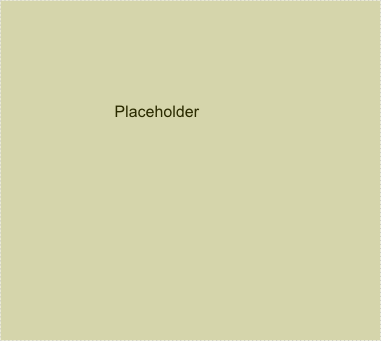
\includegraphics[width=.5\linewidth]{img/placeholder.png}
    \caption{FIGURE CAPTION.
    \label{fig:placeholder}}
\end{figure}

\begin{table}[!ht]
    \centering
    \begin{tabular}{| l | r |} \hline
Shape                           & square                    \\ \hline
Center frequency                & \SI{2.44}{\giga\hertz}    \\ \hline
Gain                            & \SI{0.625}{\dBi}          \\ \hline
    \end{tabular}
    \caption{TABLE CAPTION.
    \label{tab:placeholder}}
\end{table}

\begin{equation} \label{eq:localmarkov}
X_t \indep X_{\V\backslash (t \cup \textbf{ne}(t))} \mid X_{\textbf{ne}(t)}
\end{equation}

\TODO{SOMETHING}

% }}} sec:SECTION

% {{{ epilog

\clearpage
\addcontentsline{toc}{section}{References}
\bibliography{main}{} % main.bib
\bibliographystyle{plain}

\ifdefined\ShowGlossary
    \addcontentsline{toc}{section}{Glossary}
    \printnoidxglossary[sort=letter]
\fi

\ifdefined\ShowAppendix \begin{appendices} % {{{
    \addappheadtotoc
    \appendixpage

    \section{APPENDSEC}
    \label{appendix:APPENDSEC}

    \subsection{APPENDSUBSEC}\label{appendix:APPENDSUBSEC}
    \lstC
    \begin{lstlisting}
    // Example
    #include<stdio.h>
    main()
    {
        printf("Hello World");
    }
    \end{lstlisting}

    \section{Lists}

    \listoffigures

    \listoftables

\end{appendices} \fi % }}}

% }}} epilog

\end{document}
